%! TeX program = lualatex
\documentclass[aip,jcp, amsmath, amssymb, reprint]{revtex4-1}

\usepackage{graphicx}% Include figure files
\usepackage{dcolumn}% Align table columns on decimal point
\usepackage{bm}% bold math
\usepackage{color}
%\usepackage[mathlines]{lineno}% Enable numbering of text and display math
%\linenumbers\relax % Commence numbering lines

\usepackage[utf8]{inputenc}
\usepackage[T1]{fontenc}
%% Loads a Times-like font. You can also load
%% {newtxtext,newtxtmath}, but not {times}, 
%% {txfonts} nor {mathtpm} as these packages
%% are obsolete and have been known to cause problems.
\usepackage{mathptmx} 

\draft

\begin{document}

\title{In-silico study of DNA Mono-nucleotide Self-Assembly}
\date{\today}

\author{Mattia Trapella}
%\email[E-mail:]{ mattia.trapella@dottorandi.unipg.com}
\affiliation{Dipartimento di Fisica e Geologia, Universit\`a di Perugia, Perugia, Italia}

\author{Tommaso Bellini}
%\email[E-mail:]{ tommaso.bellini@unimi.it}
\affiliation{Dipartimento di Biotecnologie Mediche e Medicina Traslazionale, Universit\`a degli studi di Milano, Milano, Italia}
\author{Cristiano De Michele}
\email[E-mail:]{ cristiano.demichele@uniroma1.it}
\affiliation{Dipartimento di Fisica, “Sapienza” Universit\`a di Roma, Roma,Italia}

\begin{abstract}
  Origins of life are based on supra-molecular structuring
  of nucleic acid polymers in solution, which allows transfer and memory of genetic information in life. 
  Hence, study single mono-nucleotide self-assembly into DNA duplexes is crucial to understand 
  the emergence of life on earth.
  % \cite{Jia}. 
  In this work, we numerically investigated the phase behaviour of a solution of DNA
  mono-nucleotides by developing a novel, extremely coarse-grained model. Specifically, 
  we designed a model of a single nucleotide based on a semi-disk-like polyhedron decorated with attractive 
  (patchy) sites for mimicking stacking and pairing interactions. Noteworthy, 
  this model successfully captured the experimental phase behavior which has been recently studied.
  We carried out Monte Carlo simulations of patchy polyhedra by adapting algorithms borrowed 
  from computer graphics.% \cite{libccd}.
\end{abstract}

\maketitle


\section{Introduction}
Understanding the liquid crystal phase of DNA is of paramount significance for unraveling the enigma of origins of life
on earth. Understanding the self-assembly of DNA mono-nucleotides not only could shed light on the genesis of 
supra-molecular structures crucial for genetic information transfer and memory in life, but also could help the 
development/validation of theories on the emergence of life itself~\cite{Jia}. 
For example it has been argued that  liquid crystal assemblies of nucleic acids may have facilitated the formation 
of long biopolymers necessary for life. In this context, the study of DNA liquid crystals may provide 
insights into the fundamental processes behind life emergence.  \\

Recent research has demonstrated a fascinating phenomenon in the behavior of nucleic acid mononucleotide triphosphates
(dNTPs) when subjected to specific conditions: at sufficiently high concentrations and low temperatures in an aqueous
solution, these molecules undergo a liquid crystalline transition to a columnar phase~\cite{Smith}. 
These dNTPs, with an approximate length of 4 nm, can stack one on top of each other, forming longer strands and thus 
inducing the formation of the columnar phase. These experimental findings calls for 
the development of computational model able to capture and understand the observed phase behavior.
In the literature~\cite{Nguyen,C0JM02355H,Bellini} 
coarse-grained models have been proposed which approximate these filaments as hard cylinders and quasi-cylinders, each with two attractive patches. These models well describe the phase behavior of DNA duplexes (e.g. the Dickerson
dodecamer~\cite{DeMichele12}), exhibiting an isotropic, nematic and columnar phases.
Anyway, DNA mononucleotide do not form a nematic phase at temperatures and concentrations 
similar to those of DNA duplexes.
This inconsistency between experimental findings and simulations results prompts the
pursuit of a suitable numerical description of these experiments. 
The goal of the present work is precisely to develop a coarse-grained mode of dNTPs which fully accounts for the experimental 
results, which exhibit a transition from an isotropic to a columnar phase without any intermediate nematic phase and which is 
possible able to reproduce the temperature dependence of the phase boundaries.

\section{\label{sec:level1}Model and simulation details}
\begin{figure}[h!]
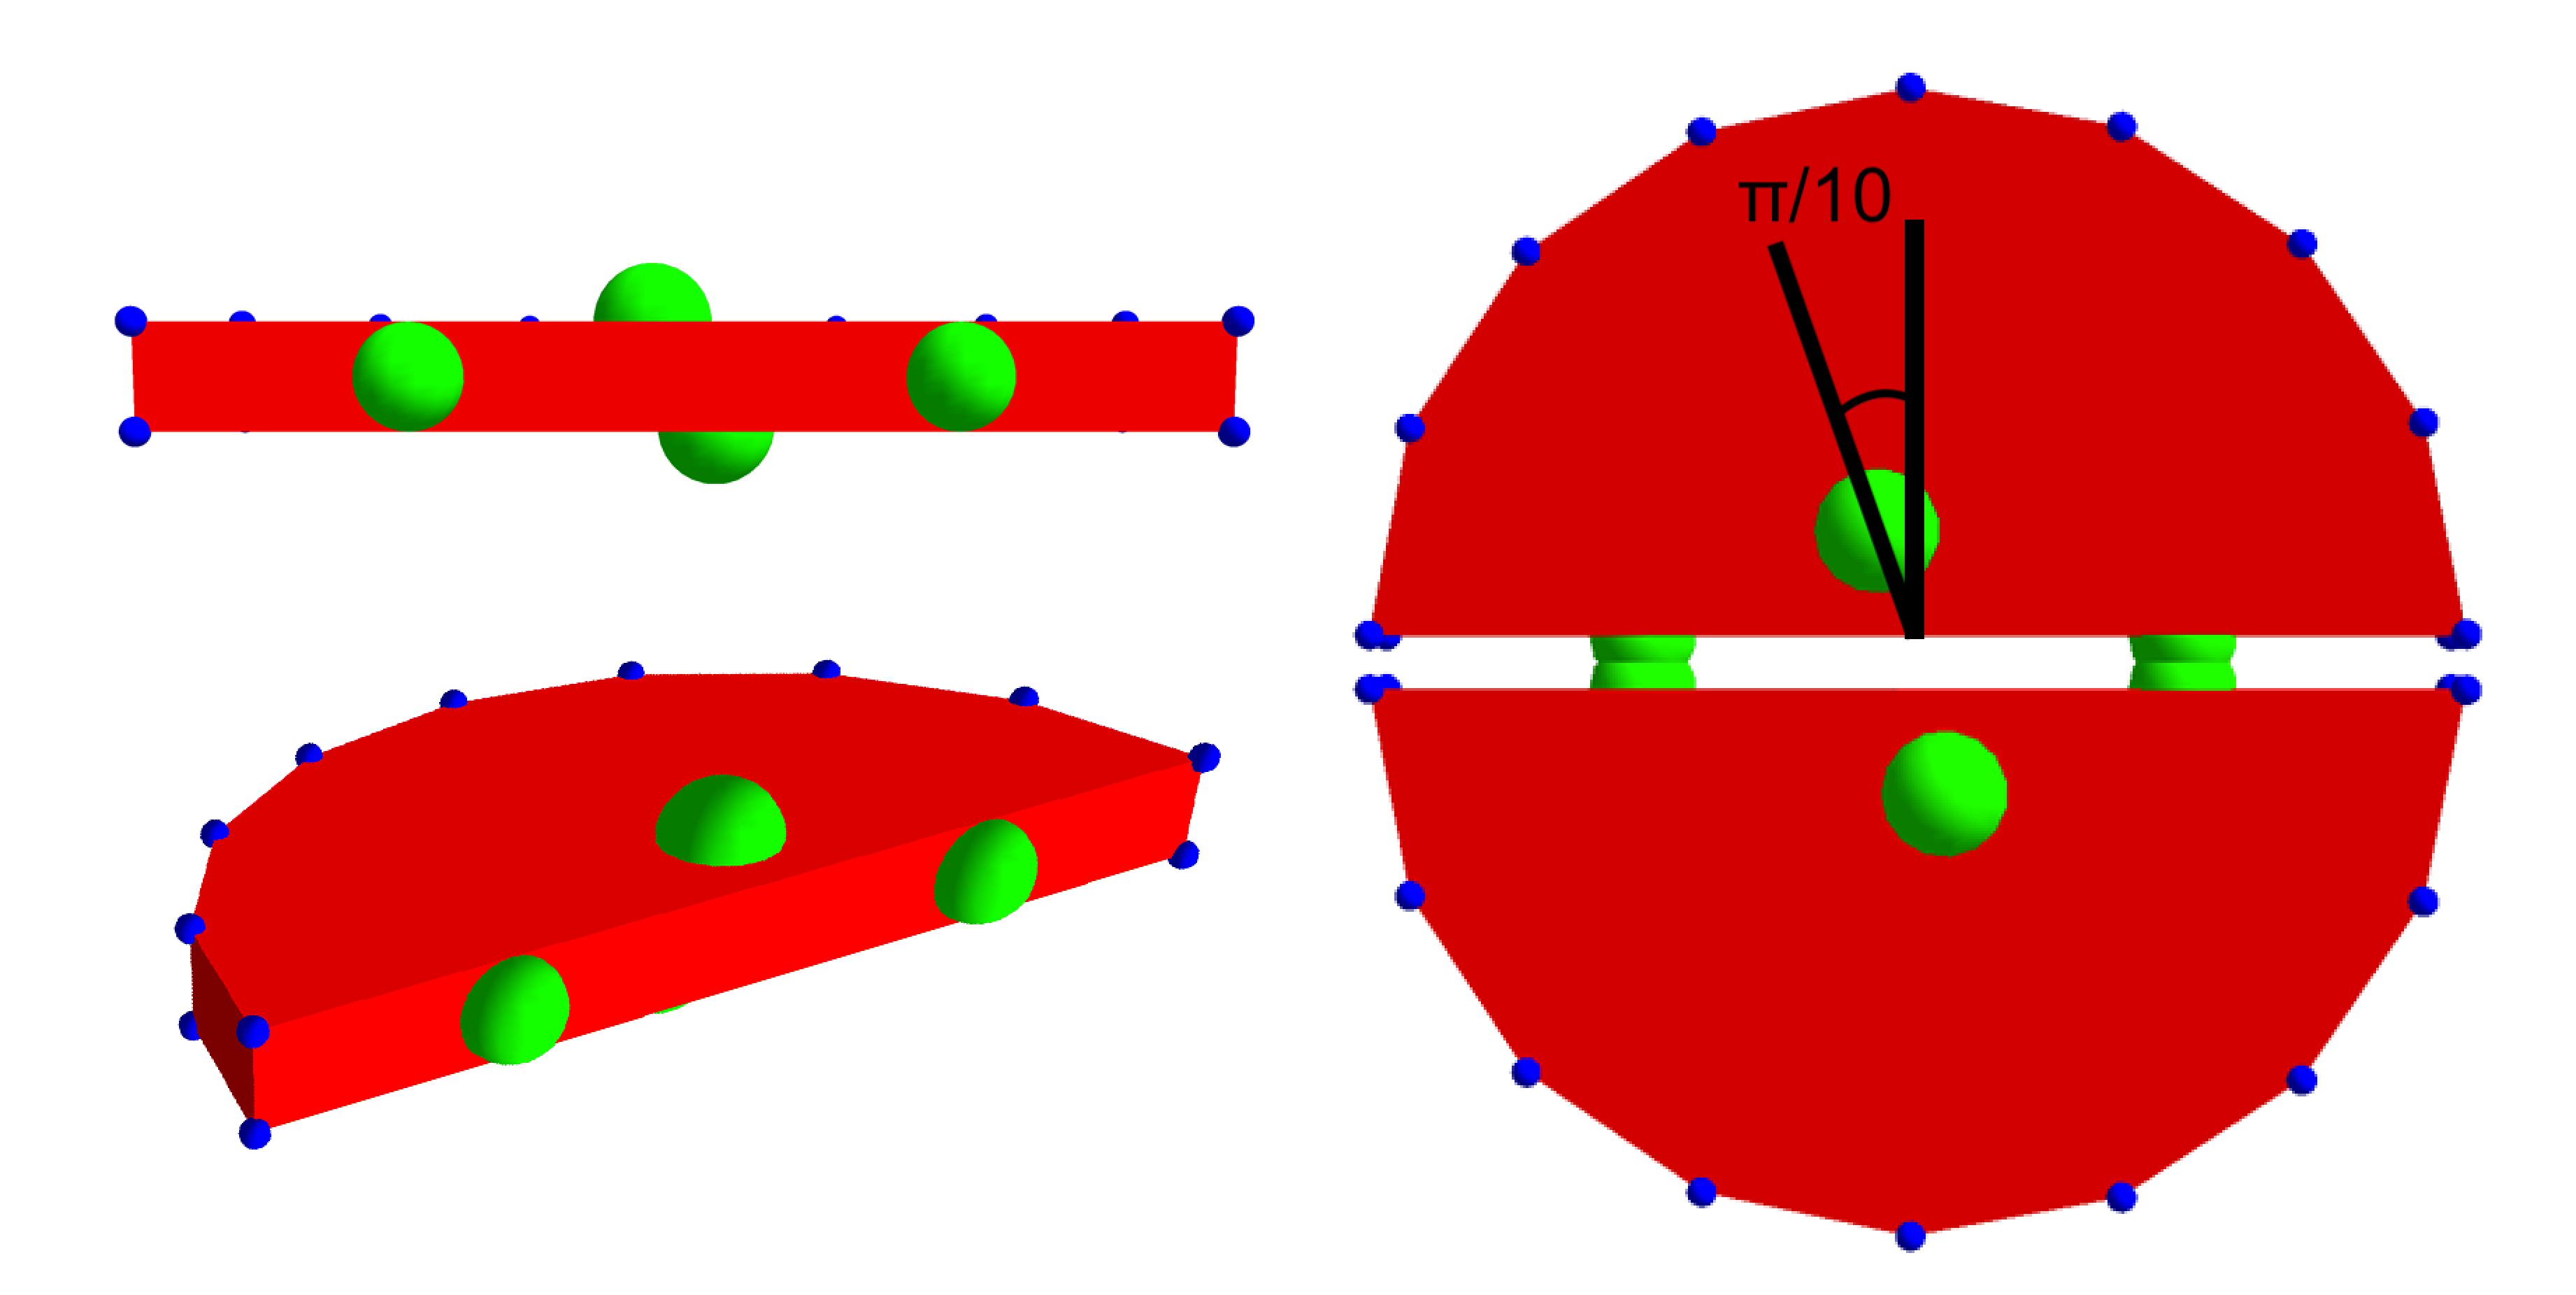
\includegraphics[width=1\linewidth]{rota.png}
\caption{\label{fig:rota} Semi-disk, that approximate the single nucleotides, with 4 attractive patches, two for stacking and two for pairing. The staking patches are rotated by $\pi/10$ so that the strand rotates on itself.}
\end{figure}
Our approach consists in modeling the dNTPs as semi-disks-like polyhedra 
featuring four distinct attractive patches. More specifically, two patches are placed along the cut
edge of the semi-disks to replicate the base-base pairing interaction, while two additional patch are located
at the center of the two bases of the semi-disk to mimic the stacking attraction between two dNTPs. 
Notably, to take into account the characteristic twist
of self-assembled DNA strands, the two stacking patches are 
placed in such a way that they give rise to their complete revolution
every 12 bases around the symmetry axis of an self-assembled DNA duplex. 
This is achieved by rotating the two patches belonging to a single semidisk by $\pi/10$ 
as shown in Figure~\ref{fig:rota}. 
% COMMENTO: se parto da una sistema di monomeri i dischi con patch 


Each semidisk is modeled as a polyhedra composed of a finite number of vertices, hence they are not exact semidisks (i.e. 
obtained by cutting in half a disk). Therefore, in the following we discuss a procedure to estimate the minimal number 
vertices to use to consider the polyhedra equivalent to exact semidisks. In this respect the goal was to have a polyhedra
which provides a physical behavior identical to that of exact semidisks. In a Monte Carlo simulation of polyhedra is needed
to have an algorithm for detecting their overlap. Since the number of vertices is not necessarily small, 
it was important to employ an efficient algorithm. After having done a comprehensive
evaluation, we found that the algorithm {\it Xenocollide}\cite{libccd} was best option, being both computationally very efficient 
and robust (i.e.~it is ensured that overlap are not missed).\\

We adjusted the model parameters to obtain reasonable values for the persistence and contour length of the self-assemble 
DNA duplexes. These adjustments include a fine-tune include fine-tune of the spatial placement and size of 
the attractive patches, as well as a refinement of the geometry and position of the stacking patches. 

\begin{figure}[h!]
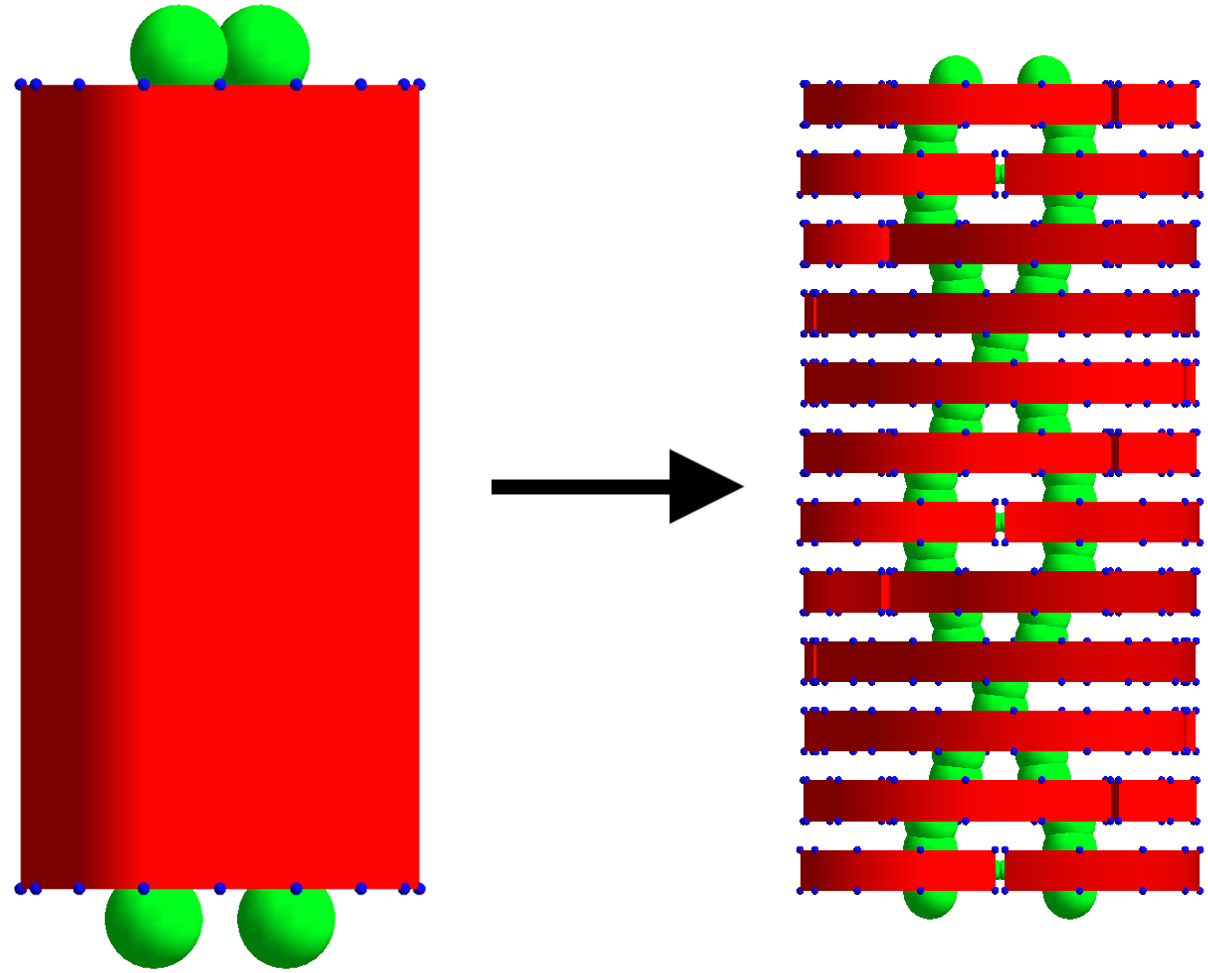
\includegraphics[width=0.7\linewidth]{sosti4.png}
\caption{\label{fig:fila} The cylinder is replaced by 24 semi-disks. the cylinder patches are rotated to match once the semi-disks are replaced.}
\end{figure}

In our simulations we first check that patchy semidisks (PSDs) selfassemble into 
cylinder-like aggregates in a small system. In Fig.XX %~\ref{fig:sdselfass}
(a) we show an initial isotropic configurations of PSD and a subsequent equilibrium 
configuration with cylinder-like aggregates. 

Since the equilibration process starting from unbonded PSDs is rather slow, 
it will take much time to equilibrate a system large enough to avoid finite size
effects, hence we use the following approach.
Equilibrium liquid crystalline phases (namely, nematic and columnar) are 
initially obtained for patchy cylinders (PHCs). 
In particular we built the whole equation of state of PHCs which exhibits
isotropic (I), nematic (N), and columnar (C) phases as illustrated in Figure 2.
Finally, we replace PHCs with PSDs and we use the resulting configurations
to start new simulations to assess their thermodynamic stability. 
Note that the adoption of four-patch cylinders ensure that by replacing
them with a set of PSDs the bonds between two distinct PSDs are preserved as shown in Figure~\ref{fig:fila}.
%%After PHCs are replaced with a set of PSDs, we also checked their stability 
%%through a NTV simulation.


\subsection{Approximation of semidisk with convex polyhedra}
Here we discuss how to approximate a semidisk with a convex polyhedron. We seek for using the minimal number of vertices
which provides accurate physical properties of the system (i.e. in this case semidisk).
Determination of an optimal number of vertices for polyhedra approximation is crucial to have an accurate physical
description while maintaining a good computational efficiency.
With \textit{Xenocollide} time to find if two polyhedra overlap scales linearly with the number of vertices.
%Limiting the number of vertices is imperative to prevent excessive simulation times, using the
%\textit{Xenocollide} algorithm, where execution time scales linearly with vertex count.
Our strategy was to build the equation of state (EOS) of hard convex polyhedra which have a cylinder-like shape and to 
compare this EOS with that of real hard cylinders.
We carried out Monte Carlo simulations in the isobaric-isothermal (NPT) ensemble for
cylinders of two different aspect ratio $X_0=L/D$, where $L$ is the length and $D$ the diameter of the cylinder. 
We also simulated cylinder-like polyhedra with the same aspect ratio and composed of 16, 24 and 32 vertices.
Before the production runs we equilibrated the system for at least $4$ million Monte Carlo steps and we check 
equilibration by inspection system volume.
\begin{figure}[h!] 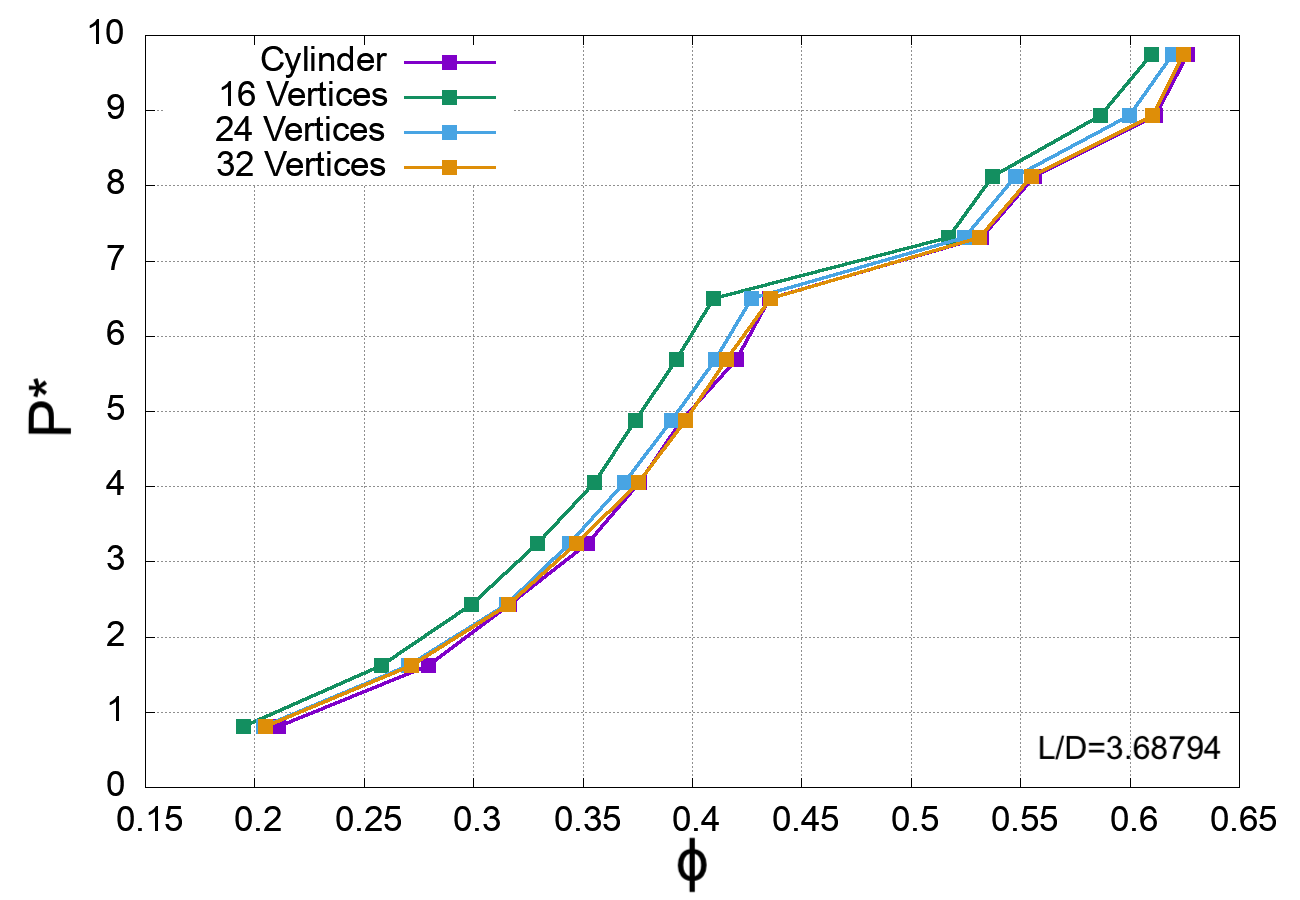
\includegraphics[width=0.9\linewidth]{cylapprox.png}
  \caption{\label{fig:cylapprox} Equation of state of cylinders with aspect ratio of $L/D=3.68794$. The equation of
  state of the cylinders is compared with their approximation to polyhedra with 16, 24 and 32 vertices.}
\end{figure}

Figure~\ref{fig:cylapprox} shows the resulting equations of state, where qualitative physical behavior is preserved for
all number of vertices. It can be noted just a slight shift of EOS towards smaller volume fractions for $V= 16$ and $24$,
while a satisfactory approximation of the EOS with that of exact cylinders is achieved with $V=32$ vertices. 
Thus, in our numerical simulations of semidisks we will use $V=16$ vertices, being a semidisk half a cylinder. 

\subsection{Stacking Free Energy}

{\color{red} COMMENTO: forse toglierei questo paragrafo o metterei tutto in appendice, poiché in fin dei conti 
  per la figura finale variamo la temperatura in un range che ci da l'accordo con gli esperimenti, ovvero
avremmo potuto fare a meno di queto mapping in temperatura.}
In this paragraph, we discuss the calculation of the stacking free energy~\cite{DeMichele12}, which is essential for
transitioning from two-patch cylinders to four-patch cylinders. 

For speeding up the equilibration process we first carried out a simulation of HCs decorated with 4 patches on thier bases and the we replace
these cylinders with patchy semidisks. An estimate of the stacking free energy to use for modeling DNA duplexes with hard cylinders 
decorated with two attractive on their bases is known as discussed in Ref.~\cite{DeMichele12}. The stacking free energy required for the
aggregation of two HCs decorated with 4 patches should be of the same order of the one for the aggregation of two HCs decorated with two patches.
Hence, here we estimate the interaction strength of the two patches on each base of each HC in such way that the stacking free energy matches with
the one of HCs decorated with two patches.

%Indeed, when replacing the cylinders with cut disks in
%nematic or columnar phases, the transition entails having one patch per base with two patches. Since the aim is to
%maintain the bonding energy unchanged, it is imperative to enforce the same stacking free energy in both systems.
Stacking free energy is defined as:
\begin{equation}
	\beta\Delta F_b=\ln \bigg[2\frac{\Delta(T)}{v_d}\bigg]
	\label{deltaf}
\end{equation}

where:
\begin{equation}
\label{deltat}
	\Delta(T)=\frac{1}{4}\bigg\langle \int_{V_b} [e^{-\beta V(\textbf{r}_{12}, \Omega_1, \Omega_2)}-1]d\textbf{r}_{12}\bigg\rangle
\end{equation}

With $\textbf{r}$ denoting the vector connecting the centers of mass of particle 1 and particle 2, $\Omega_i$
representing the orientation of the i-th particle, and $\langle\ldots\rangle$ indicating the average taken over all
directions, $v_d$ stands for the volume of the considered object, while $V_b$ represents the bonding volume. The
calculation of $\Delta (T)$, in the case of attractive patches, simplifies and for two patches per base one has 

%because it suffices to calculate the
%probability of obtaining a single bond and that of obtaining a double bond, then weigh them respectively by $\exp(\beta
%U_0)$ and $\exp(2\beta U_0)$. Consequently, the equation for $\Delta (T)$ in Eq.~\eqref{deltat} becomes:
\begin{equation}
\label{deltat2}
	\Delta(T)=\frac{1}{4N}\big( N_1(e^{\beta u_0}-1)+N_2(e^{2\beta u_0}-1)\big)
\end{equation}

where $u_0$ is the bonding energy, $N$ indicates the total number of insertions, $N_1$ and $N_2$ represent the occurrences of having one and two
bonds, respectively. 

Through a Monte Carlo algorithm, one can estimate $\Delta(T)$
%Subsequently, a program is developed to insert a cylinder at the origin and then insert a second
%cylinder with random position and orientation inside a box with dimensions sufficient to contain both. The number of
%bonded patches is verified for each insertion, with a total of 5 billion insertions performed. Following the
%simulations, the reduced temperature, defined as 
and find $T^*_{2 patch}=k_B T_{2 patch}/U_0$, such that ${\Delta F_b}^{1 patch}(T^*_{1 patch})=\Delta F_b^{2 patch}(T^*_{2 patch})$, 
which is then use ad a first estimate of stacking energy to use in the simulations.
%in simulations of cut disks to attain %the same stacking free energy.

\subsection{EOS cylinder with 4 patches}
Dickerson dodecamers can be modeled as patchy hard cylinders (PHCs) decorated with two sticky patches on their 
bases~\cite{DeMichele12}. In this case the phase behavior includes isotropic, nematic and columnar phases.
As we anticipated in the introduction, to reduce computational times we first obtain equilibrium configurations
by simulating PHCs and then we replace PHCs with a set of $24$ PSDs. Afterward we make PSDs equilibrate to check the stability
of I, N and Col phases. The only caveat is that we used PHCs decorated with two patches per base, chosen in such a way 
that stacking free energy is identical to that of PHCs with one patch per base. 
Hence, we built the EOS of PHCs with four patches and then we select I, N e Col configurations to start PSDs simulations
where PSDs replace PHCs.

The EOS of PHCs is shown in Figure~\ref{fig:eos1}, where to distinguish the various phase we inspect the radial distribution function we make use of the 
nematic $S$ and hexagonal $\psi_6$ order parameters.

The namatic order parameter $S$ is defined as the largest eigenvalue of the order tensors, i.e.

where...
while $\psi_6$ is defined as:

%isotropic phases are considered those with nematic order parameter $S<0.15$, and columnar phases are considered those
%with hexagonal order parameter $\psi_6 > 0.3$. The nematic order parameter $S$ and the hexagonal order parameter $\psi_6
%$ are calculated respectively by: 
\begin{equation}  
\label{pordnem}
S= \bigg\langle \frac{3}{2} \cos^2\theta - \frac{1}{2} \bigg\rangle; \; \; \; \; \; \; \; \; \; \langle \psi_6\rangle=\bigg\langle \frac{1}{N} \sum_{i=1}^N \frac{1}{n(i)} \sum_{j=1}^{n(i)}e^{6i\theta_{ij}} \bigg\rangle
\end{equation}
Concerning the radial distribution function is defined as follows....

\begin{figure}[h!]
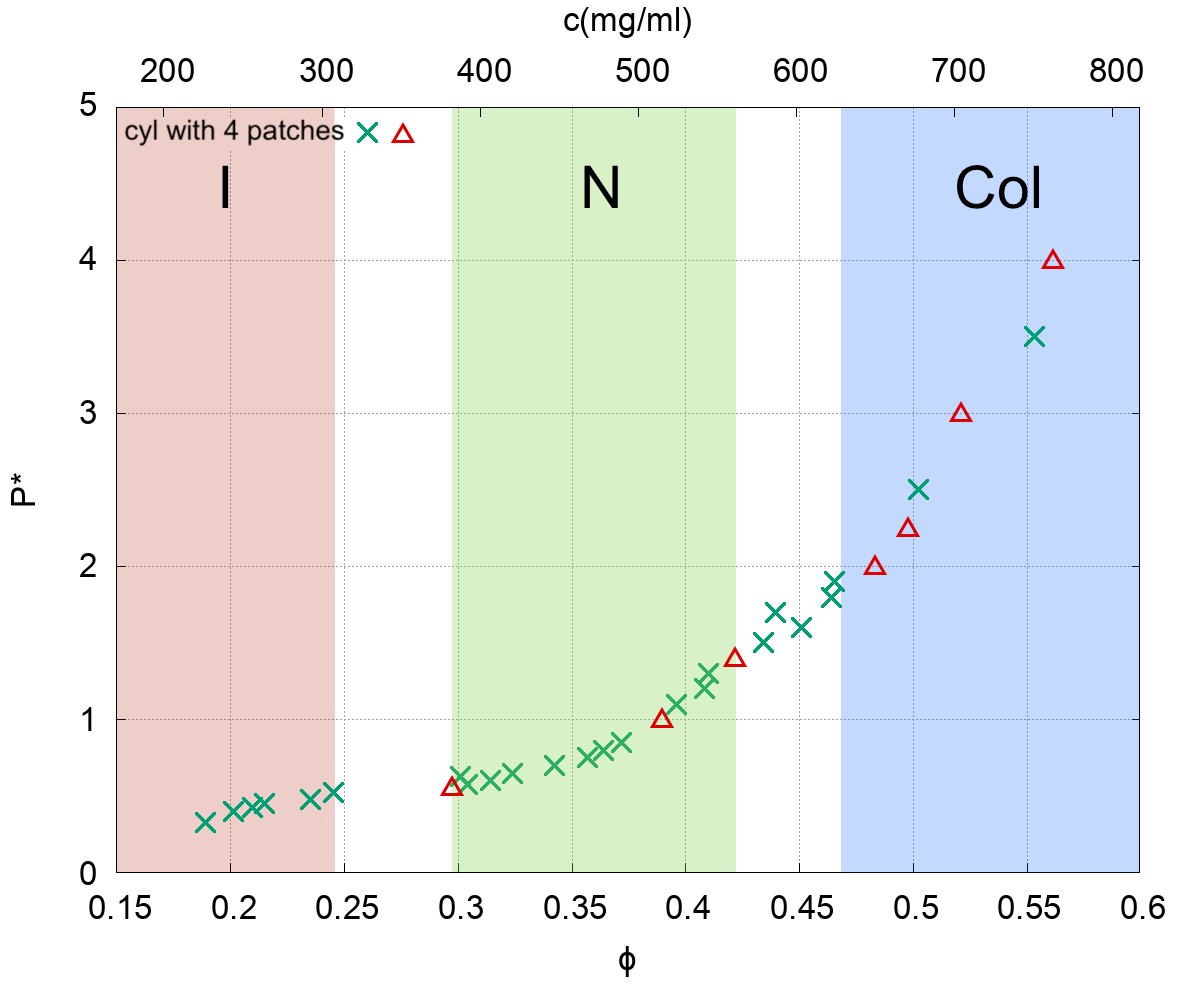
\includegraphics[width=0.86\linewidth]{eos.png}
\caption{\label{fig:eos1} Equation of state for cylinders with aspect-ratio $X_0=2$ and 2 attractive patches per base. The simulations employ $N = 180$ particles and evolve over 4 million Monte Carlo steps. The symbols in red represent the simulations whose finale configuration are used for simulating PSDs after the replacement of HCs.}
{\color{red} nella leggenda vanno messe entrambi i simboli e questi è meglio che siano diversi
e non solo di diverso colore. Usiamo dei cerchi per le configurazioni da usare per i PSDs.}
\end{figure}

The discrepancies {\color{red} COMMENTO: discrepancies tra cosa? non capisco...} observed in the equation of state can be ascribed to the small number ($N=180$) of particles employed in the simulations; specifically. We used this number of particles
to keep simulation times small, since each PHCs is replaced with $24$ semidisk, thus making the total number of PSDs to simulate equal to $4320$.

\section{\label{exp}Experimental methods}

\section{\label{Results}Results}
To verify the stability of the nematic and columnar phases, by substituting the cylinders with semi-disks filaments, NVT
simulations are performed. 
This replacement has to be done without introducing overlaps between PSDs, hence
the filament must be entirely contained within the original cylinder. Moreover,
the distance between the paired bases of the filament is chosen in such a way that the final 
height matches that of the original cylinder. Additionally, the filament is constructed by introducing a rotation of $\pi/5$, between successive base
pairs, to ensure that the stacking patches are all bonded. 
Figure~\ref{sosti1} shows a nematic phase of HCs with four patches before (a) and after (b)
replacing HCs with PSDs for $P^*=0.55$. 

\begin{figure}[h!]
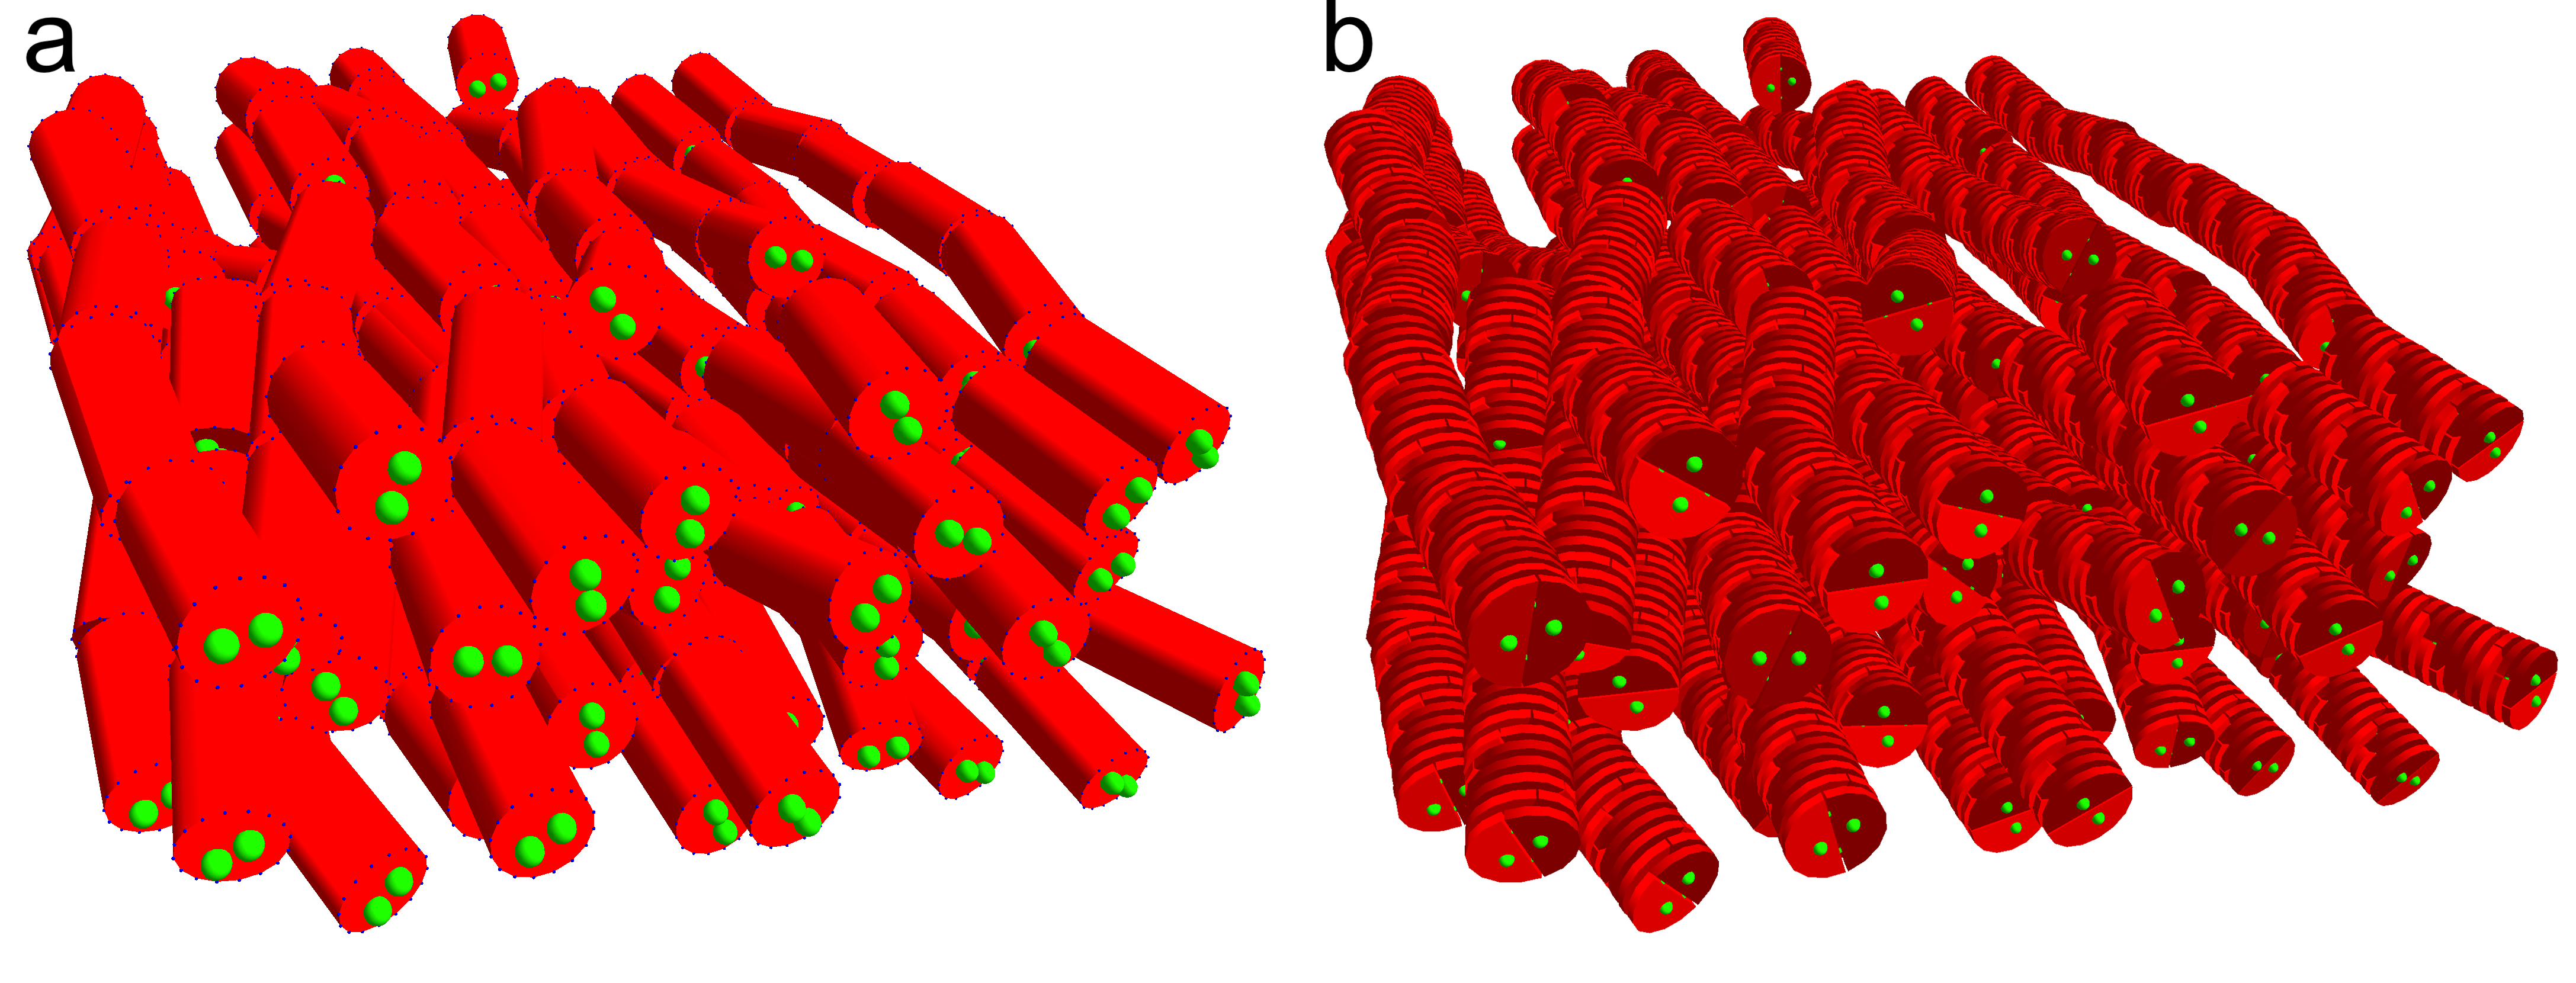
\includegraphics[width=0.9\linewidth]{sosti1.png} 
\caption{\label{sosti1} (\textbf{a}) Nematic phase with cylinders at pressure $P^*=0.55$. (\textbf{b}) Nematic phase after replacement of HCs with PSDs. } 
\end{figure} 

{\color{red} COMMENTO: Questo va spostato nella sezione sul modello}
We now discuss how to choose the stacking and pairing energies. Experimentally, the stacking interacti
strength is much larger than the pairing interaction strength. 
Hence, in our model we set a pairing energy equal to half of the stacking energy.

%However, this difference depends on various factors,
%such as the solution in which the DNA filaments are suspended. Consequently, the same energy is assigned to both
%pairing and stacking bonds. 
%This decision is made because if the phase dissolution occurs even under these conditions,
%it will certainly happen with weaker pairing bonds. 
{\color{red} COMMENTO: non ho capito la logica con cui l'energia di pairing è stata assunta
uguale a quella di stacking}
%To achieve the same energy for stacking and pairing bonds,
%considering that pairing bonds consist of two patches, the depth of the pairing patch well is halved.\\
As initial configuration for simulating PSDs we used those corresponding to the circles in Fig.~\ref{fig:eos1}.
\begin{figure}[h!]
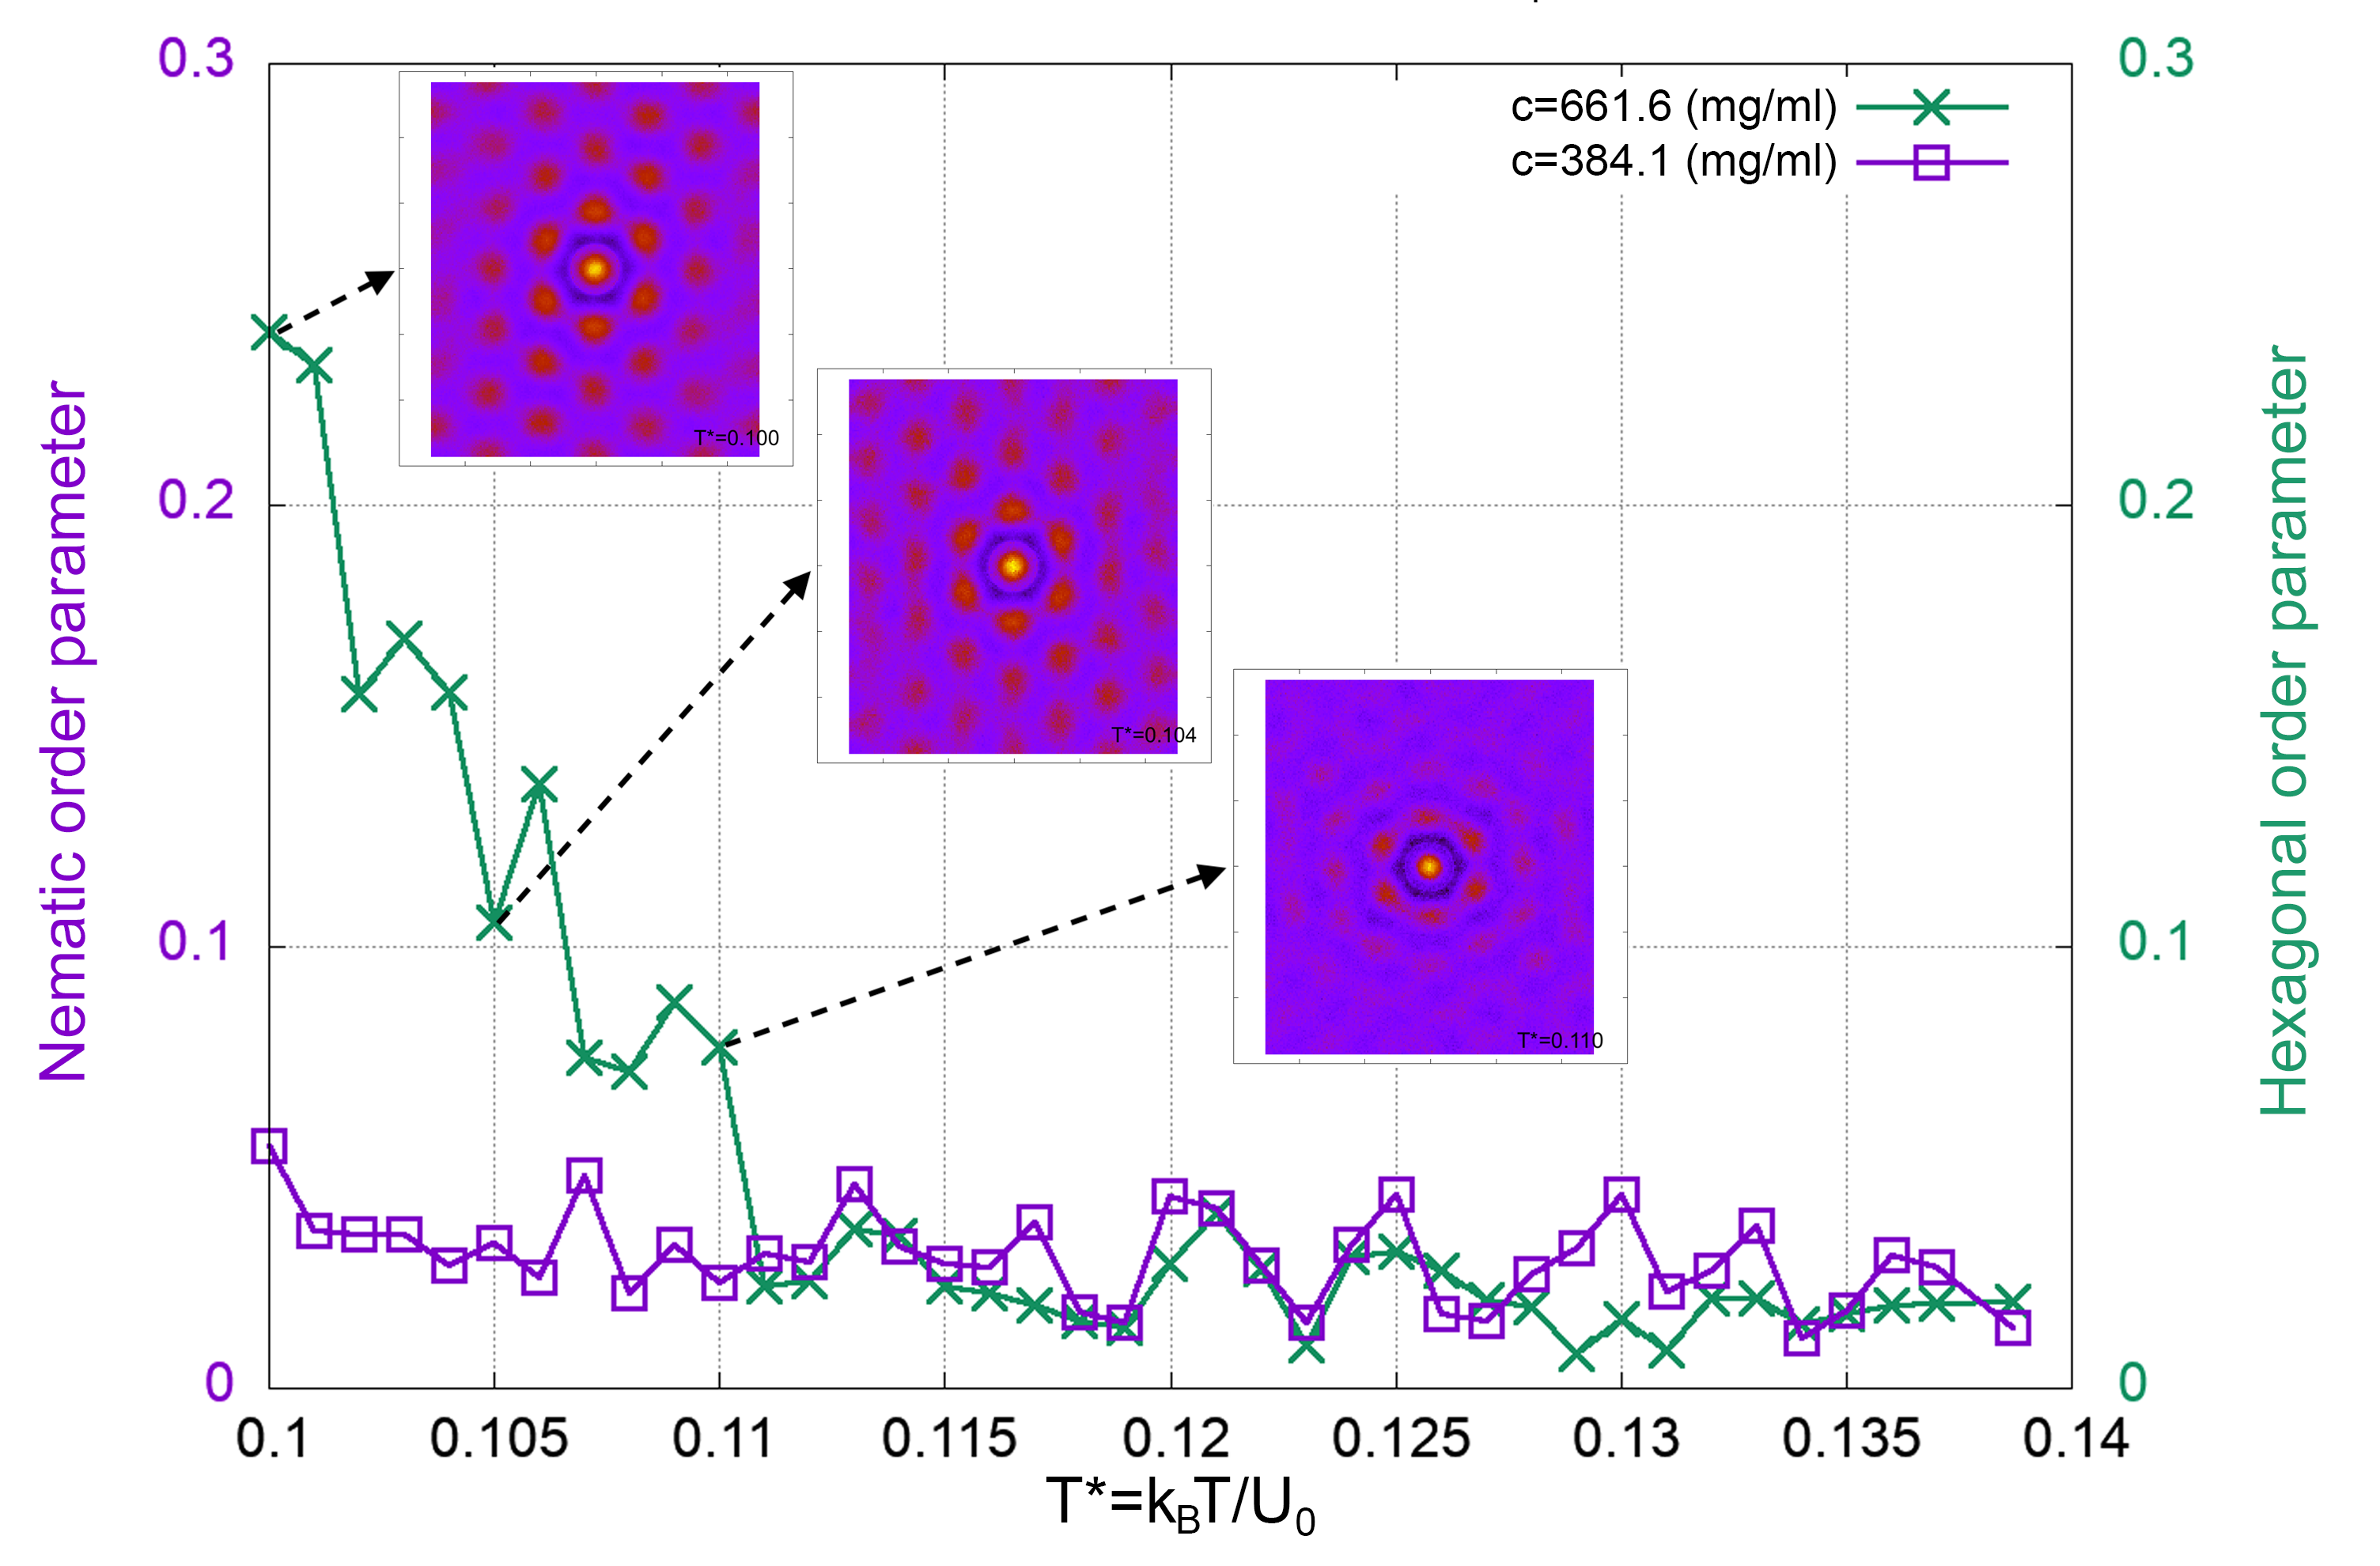
\includegraphics[width=0.99\linewidth]{par.png}
\caption{\label{fig:par} In purple, the nematic order parameter of the simulations that started from nematic phases at volume fraction $\phi=0.357$. In green the hexagonal order parameter of the simulations that started from columnar phases t volume fraction $\phi=0.483$. The graph shows the persistence of columnar phases, also highlighted by the graphs of the pair distribution function, and the dissolution of initially nematic phases.}
\end{figure}


%Three nematic phases and four columnar phases of cylinders with different volume fractions, and thus concentrations,
%are selected as indicated in red in Figure~\ref{fig:eos1}, then the cylinders are replaced by filaments of 12 pairs of
dNTPs and their stability are studied by carrying out a Monte Carlo NVT simulation at various temperatures $T^*=[0.10:0.15]$
for each starting configuration. We first note that for all temperatures investigated, the initially nematic phases are never stable and system always become isotropic, whereas the initially columnar phases are stable at low temperatures.  

 Figure~\ref{fig:par} shows the nematic and columnar order parameters for two starting configurations, one nematic and the other one columnar. In this figure we also show the pair 
 distribution functions of the columnar case on the plane orthogonal to the nematic axis; note the worsening of the hexagonal ordering as the temperature increases.


\subsection{Comparative Analysis of Experimental and Simulation Results}

Here we compare simulations results with experimental findings on dTTP/dATP mononucleotides~\cite{Smith}.
We expressed system concentration $c$ of computer simulations in mg/ml, where the conversion 
from volume fraction $\phi$ to concentration $c$ in mg/ml can be obtained as follows

\begin{equation}
	c=\frac{N}{V}m_N
	\label{conc}
\end{equation}
where $N$ represents the number of semi-disks within the simulation box's volume $V$, and $m_N$ denotes the molecular mass of a single nucleotide, measured in Daltons ($Da$). For dTTP and dATP filaments, the molecular masses are $m_N=482.2\; Da$ and $m_N=491.2\; Da$ respectively. Since the experimental results refer to a mixture of dTTP and dATP filaments, we consider for
the conversion the average molecular masses of the two species, i.e. $m_N=486.7\; Da$. 
Figure~\ref{fig:wide}, shows experimental 
findings of dATP/dTTP filaments~\cite{Smith} together with Monte Carlo simulation results of PSDs. 
Above a concentration of 600 mg/ml simulations exhibit a phase transition from I to Col, whereas at lower concentration
system is isotropic for all temperatures investigated. This behavior mathes the experimental results and more interestingly
our model seems to have the right temperature dependence concerning the phase boundaries.

\begin{figure*}[t!] 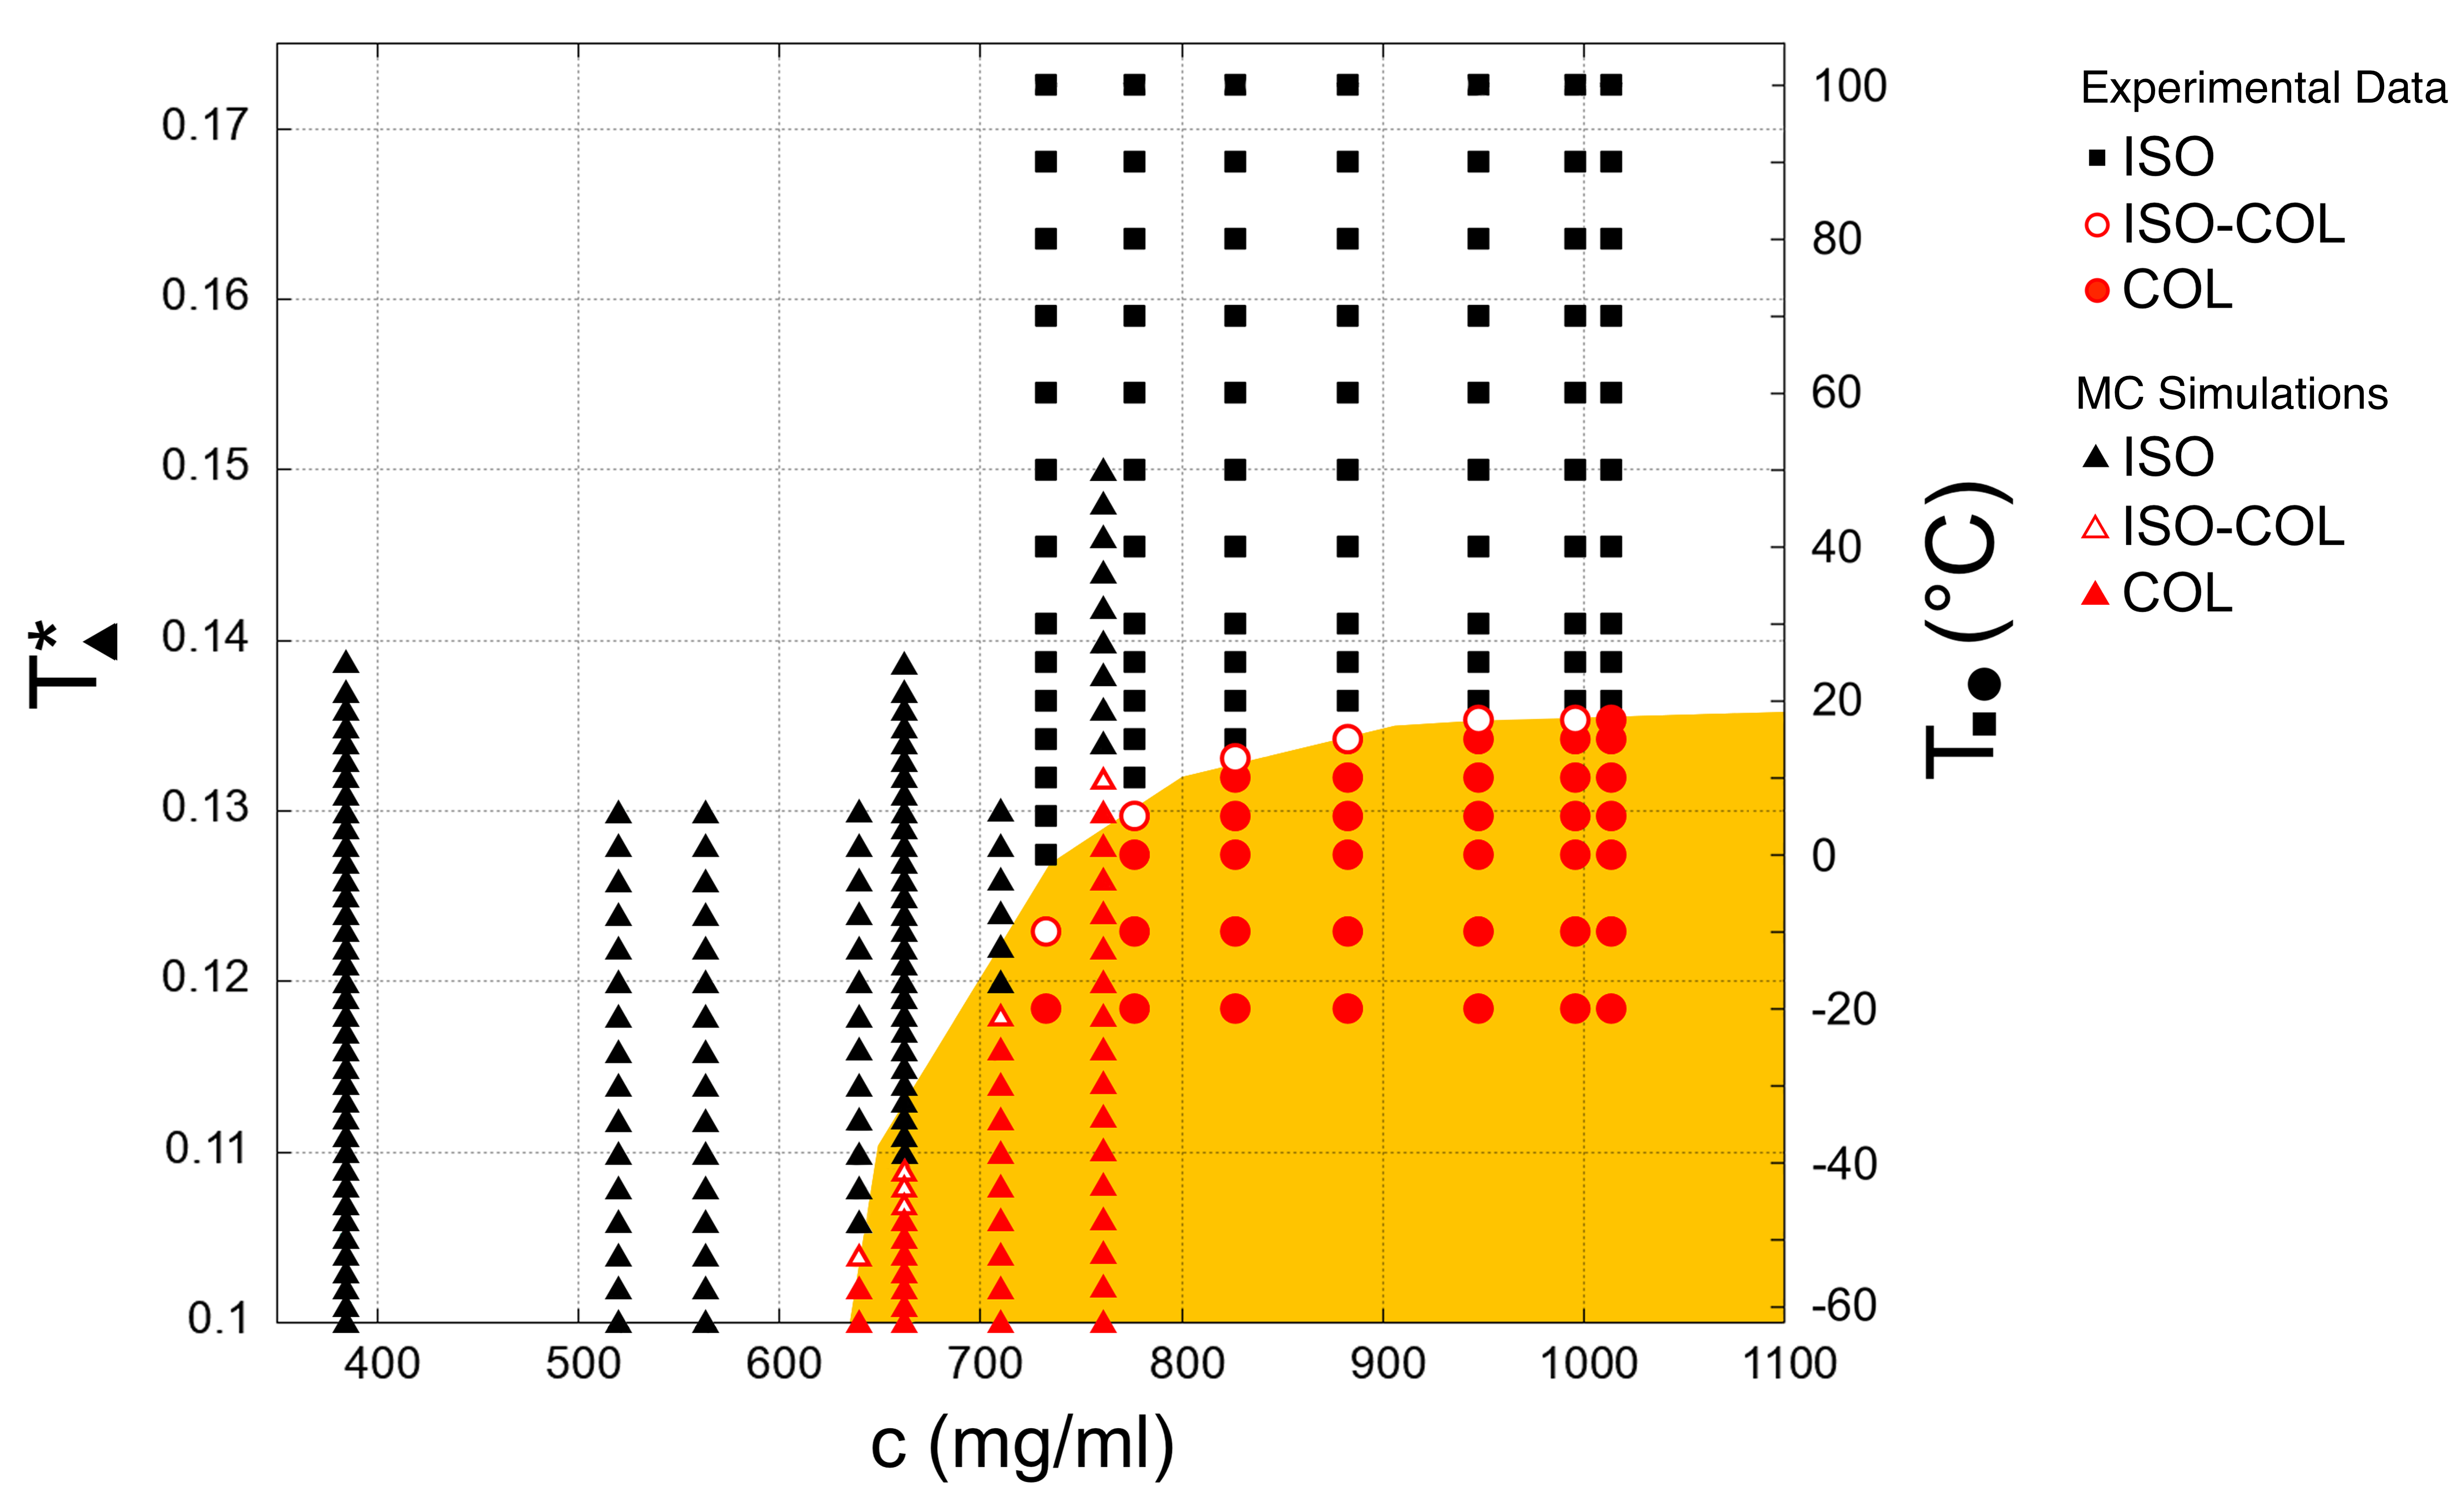
\includegraphics[width=0.7\linewidth]{finaleeng.png} \caption{\label{fig:wide}Phase diagram of
    dTTP/dATP DNA strands. The square and round symbols refer to the experimental results while the triangular symbols
  refer to the results obtained from the simulations. The orange area indicates where the columnar phase is present.}
\end{figure*}



The absence of a nematic phase in the phase diagram of PSDs can be rationalized through Wertheim-like
theory developed in Refs.~\cite{Macromol12}.Indeed, if we consider aggregating bifunctional HCs of 
length $L$ and diameter $D$ the will form a polydisperse set of polymers (e.g.~see~\cite{DeMichele12}).
We start noting that, in our present case, the self-assembled structure formed by PSDs can be regarded 
as a set of $12$ disks formed each by two paires PSDs, where the stacking free energy of two disks is equal to 
that of two PHCs with four attractive patches.

According to the theory, the average number $M$ of HCs belonging to a polymer at a given concentration 
and temperature in the isotropic phase is:
\begin{equation}
M(\phi, T) = \frac{1}{2}\left( 1 + \sqrt{1 + 4 \phi e^{k_I \phi \eta(\phi)+\beta {\Delta F}_b}} \right) 
\end{equation}
where $k_I$ is a geometric factor that does not depend on HC length $L$, 
$\eta(\phi) = \frac{1}{4} \frac{4-3\phi}{{(1-\phi)}^2}$ is the Parsons-Lee factor
and ${\Delta F}_b$ is the stacking free energy.
If we replace each HC with a set of $N_{sd}$ disks of diameter $D$ length $L/N_{sd}$, whereas the stacking energy between two 
disks is still ${\Delta F}_b$, we can expect $M$ to be unchanged. Anyway, the average contour length ${\cal L}$
is now $\frac{L}{N_{sd}}*M$ while in the previous case it was $\frac{L}{M}$.
Hence the average contour length of polymers becomes $N_{sd}$ times shorter. 
This means that at a given temperature IN transition shifts to much higher concentrations, if we consider HCs with smaller $L$
, thus making it hindered by the columnar phase.


{\color{green}COMMENTO: spiegare con teoria di Wertheim il comportamento osservato, ovvero
l'assenza della fase colonnare}


% TODO: sono arrivato qui
\section{\label{Dis}Conclusions}
% work on this
Our study presents a novel coarse-grained model that successfully elucidates the liquid crystal phase behaviour of dTTP/dATP nucleotide solutions. By employing semi-disk-like polyhedra decorated with four attractive patches to mimic stacking and pairing interactions, our model accurately replicates experimental observations of columnar phases without transitioning into nematic phases, a discrepancy previously encountered in computational simulations. Through meticulous adjustments and validations, including the calculation of Stacking free energy and substitution processes, our model demonstrates robustness in capturing the intricate behaviours of DNA nucleotides. Furthermore, our simulations offer insights into the stability of nematic and columnar phases under varying concentrations and temperatures. Notably, the stability of columnar phases at low temperatures corroborates experimental findings and underscores the predictive capability of our model. The comparison between simulation results and experimental data on dTTP/dATP filaments further validates the efficacy of our approach, highlighting concordance in phase transitions observed at different concentrations. \\

Overall, our study not only advances our understanding of liquid crystal phase behaviour in DNA nucleotide solutions but also underscores the potential of computational modelling in elucidating complex molecular phenomena. Future research endeavours may leverage our coarse-grained model to explore additional nucleotide systems and unravel further intricacies underlying liquid crystal phase transitions in nucleic acid polymers.


\bibliography{semidisks}
\end{document}
